\documentclass{article}
\usepackage{graphicx}
\usepackage{pgfplots}
\usepackage{subcaption}
\usetikzlibrary{patterns}
\pgfplotsset{compat=1.17}

\begin{document}

\begin{figure}[h]
    \centering
    \begin{subfigure}[b]{0.45\textwidth}
        \centering
        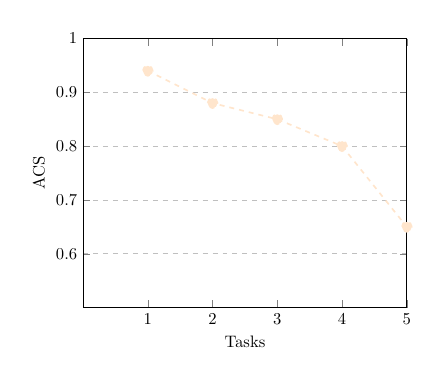
\begin{tikzpicture}[scale=0.6]
            \begin{axis}[
                xlabel={Tasks},
                ylabel={ACS},
                ymin=0.5, ymax=1.0,
                xmin=0, xmax=5,
                xtick={1,2,3,4,5},
                ytick={0.6,0.7,0.8,0.9,1.0},
                legend pos=south west,
                ymajorgrids=true,
                grid style=dashed,
            ]
            \addplot[
                color=orange!20!white,
                mark=*,
                mark options={fill=orange!20!white, scale=1.5},
                line width=1pt,
                dashed
            ]
            coordinates {
                (1,0.94)
                (2,0.88)
                (3,0.85)
                (4,0.80)
                (5,0.65)
            };
            \end{axis}
        \end{tikzpicture}
        \caption{CIFAR10}
        \label{fig:cifar10}
    \end{subfigure}
    \hfill
    \begin{subfigure}[b]{0.45\textwidth}
        \centering
        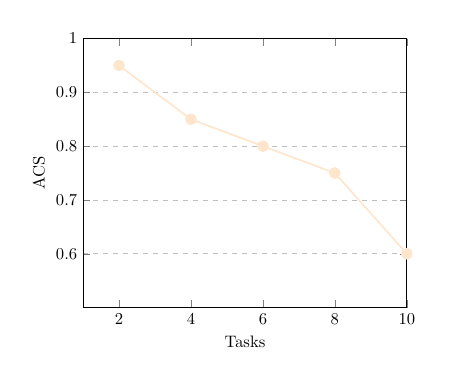
\begin{tikzpicture}[scale=0.6]
            \begin{axis}[
                xlabel={Tasks},
                ylabel={ACS},
                ymin=0.5, ymax=1.0,
                xmin=1, xmax=10,
                xtick={2,4,6,8,10},
                ytick={0.6,0.7,0.8,0.9,1.0},
                legend pos=south west,
                ymajorgrids=true,
                grid style=dashed,
            ]
            \addplot[
                color=orange!20!white,
                mark=*,
                mark options={fill=orange!20!white, scale=1.5},
                line width=1pt,
            ]
            coordinates {
                (2,0.95)
                (4,0.85)
                (6,0.80)
                (8,0.75)
                (10,0.60)
            };
            \end{axis}
        \end{tikzpicture}
        \caption{CIFAR100}
        \label{fig:cifar100}
    \end{subfigure}
    \caption{}
    \label{fig:acs_comparison}
\end{figure}

\end{document}